% WSCG sample document 
%
% based on Gabriel Zachmann's sample
% http://zach.in.tu-clausthal.de/latex/
%
% modified Apr 2012 to match WSCG Word template
%
\documentclass[twoside,twocolumn,10pt]{article}



%%%%%%%%%%%%%%%%%%%%%%%%%%%%%%%%%%%%%%%%%%%%%%%%%%%%%%%%%%%%%%%%%%%%%%%%%%%%%
%                             Packages

\usepackage{wscg}           % includes a number of other packages (e.g., myalgorithm)
\RequirePackage{ifpdf}
\ifpdf
 \RequirePackage[pdftex]{graphicx}
 \RequirePackage[pdftex]{color}
\else
 \RequirePackage[dvips,draft]{graphicx}
 \RequirePackage[dvips]{color}
\fi


\usepackage{nopageno}       % no page numbers at all; uncomment for final version

\usepackage{subfig}
\usepackage{graphicx}
\usepackage[justification=centering]{caption}
\usepackage{amsmath}
\usepackage[linesnumbered,ruled]{algorithm2e}
\usepackage[english]{babel}
\usepackage{enumitem}
%%%%%%%%%%%%%%%%%%%%%%%%%%%%%%%%%%%%%%%%%%%%%%%%%%%%%%%%%%%%%%%%%%%%%%%%%%%%%
%                                Title

\title{MAELab: a framework to automatize landmark estimation}

\author{
  \hspace{-0.1\textwidth}
  \parbox{0.2\textwidth}{\centering
    LE Van \\
    Linh\\[1mm]
LaBRI-CNRS 5800\\
ITDLU, Dalat Univ-V
linhlv@dlu.edu.vn/ van-linh.le@labri.fr
}
\hspace{0.02\textwidth}
\parbox{0.2\textwidth}{\centering
BEURTON-AIMAR Marie\\[1mm]
LaBRI-CNRS 5800\\
Bordeaux University\\
33400 Talence-F\\
beurton@labri.fr
}
\hspace{0.02\textwidth}
\parbox{0.25\textwidth}{\centering
KRAHENBUHL \\Adrien\\[1mm]
LaBRI-CNRS 5800\\
Bordeaux University\\
33400 Talence-F\\
adrien.krahenbuhl@labri.fr
}
\hspace{0.02\textwidth}
\parbox{0.18\textwidth}{\centering
PARISEY\\ Nicolas\\[1mm]
IGEPP\\
INRA 1349\\
35653 Le Rheu-F\\
nparisey@rennes.inra.fr
}
}

%%%%%%%%%%%%%%%%%%%%%%%%%%%%%%%%%%%%%%%%%%%%%%%%%%%%%%%%%%%%%%%%%%%%%%%%%%%%%
%                          Hyperref


% no hyperlinks
\usepackage{url}
\urlstyle{tt}

% Donald Arsenau's fix for missing kerning of "//" and ":/"
\makeatletter
\def\Uslash{\mathbin{\mathchar`\/}\@ifnextchar{/}{\kern-.15em}{}}
\g@addto@macro\UrlSpecials{\do \/ {\Uslash}}
\def\Ucolon{\mathbin{\mathchar`:}\@ifnextchar{/}{\kern-.1em}{}}
\g@addto@macro\UrlSpecials{\do : {\Ucolon}}
\makeatother




%%%%%%%%%%%%%%%%%%%%%%%%%%%%%%%%%%%%%%%%%%%%%%%%%%%%%%%%%%%%%%%%%%%%%%%%%%%%%
%                                Document


\begin{document}

\twocolumn[{\csname @twocolumnfalse\endcsname

\maketitle  % full width title


\begin{abstract}
\noindent  Phenotype of beetle species are characterized by informations like
  age, sex, morphological criteria or environmental parameters. Biologists are
  used to proceed to manual measurements in case of
  analysis at macro level as for example tissues or animal members.
  They can directly measure the geometrical characteristic of elements on the body of the animal: length,
  width, diameter, angles, \ldots Another way to obtain morphological
  measures is to take pictures of
  the members and to apply image processing algorithms. In order to
  evaluate a population of beetles from Brittany lands, a collection of
  293 beetles has been built. For each beetle, biologists took images of the left
  and right mandibles. A set of landmarks has been manually located: 16 for the left mandibles and and 18 for the right ones.
  They constitute
  the ground truth to evaluate the automatically estimated landmarks. In a previous
  work \cite{leestimating}, we have shown that the Probabilistic Hough Transform (PHT)
  is efficient to compute the centroid position of the mandible.
  If the goal is to consider more precisely
  the position or the geometry of the landmark areas, the results are not
   accurate enough to consider the replacement of manual landmarks by the automatically estimated landmarks. In this
   paper, we propose a method to improve the previous
   segmentation algorithm using the Canny algorithm. Moreover, we propose a registration
   procedure based on an Iterative Principal Component Analysis.
   Finally, the landmarks are located using
   a SIFT descriptor computed in the landmarks area of the model image.
   The complete workflow is implemented in MAELab, freely available as library on a GitHub website.
\end{abstract}

\subsection*{Keywords}
Morphology, image registration, detector/descriptor, SIFT, beetle, mandible
\vspace*{1.0\baselineskip}
}]



%%%%%%%%%%%%%%%%%%%%%%%%%%%%%%%%%%%%%%%%%%%%%%%%%%%%%%%%%%%%%%%%%%%%%%%%%%%%%


\section{Introduction}

\copyrightspace
In biology, the morphological analysis is widely used to detect the inter-organisms variations.
It allows to determine the evolution of an organism family and to classify these
organisms. Especially in agriculture, morphology is one of the best ways
to learn about the evolution of the beetle on crops (see Fig. \ref{figparts}).

The morphology methods may be divided into groups considering the features used
such as shape, structure, color, pattern or size of the
object. In order to study the potential links between these
characteristics and agricultural ecosystems, a set of beetles has been
analyze to collect a lot of informations. Their sex, place where they were
found and agricultural practices in each field were recorded. For each
beetle, the morphometric landmarks has been manually identified on the mandible images.
The morphometric landmarks are precise points defined by biologists. Landmarks are
used in many biological studies and are currently included
into the classification procedures.

\begin{figure}[h]
\centering
\subfloat[Left mandible]{\label{figrbox2}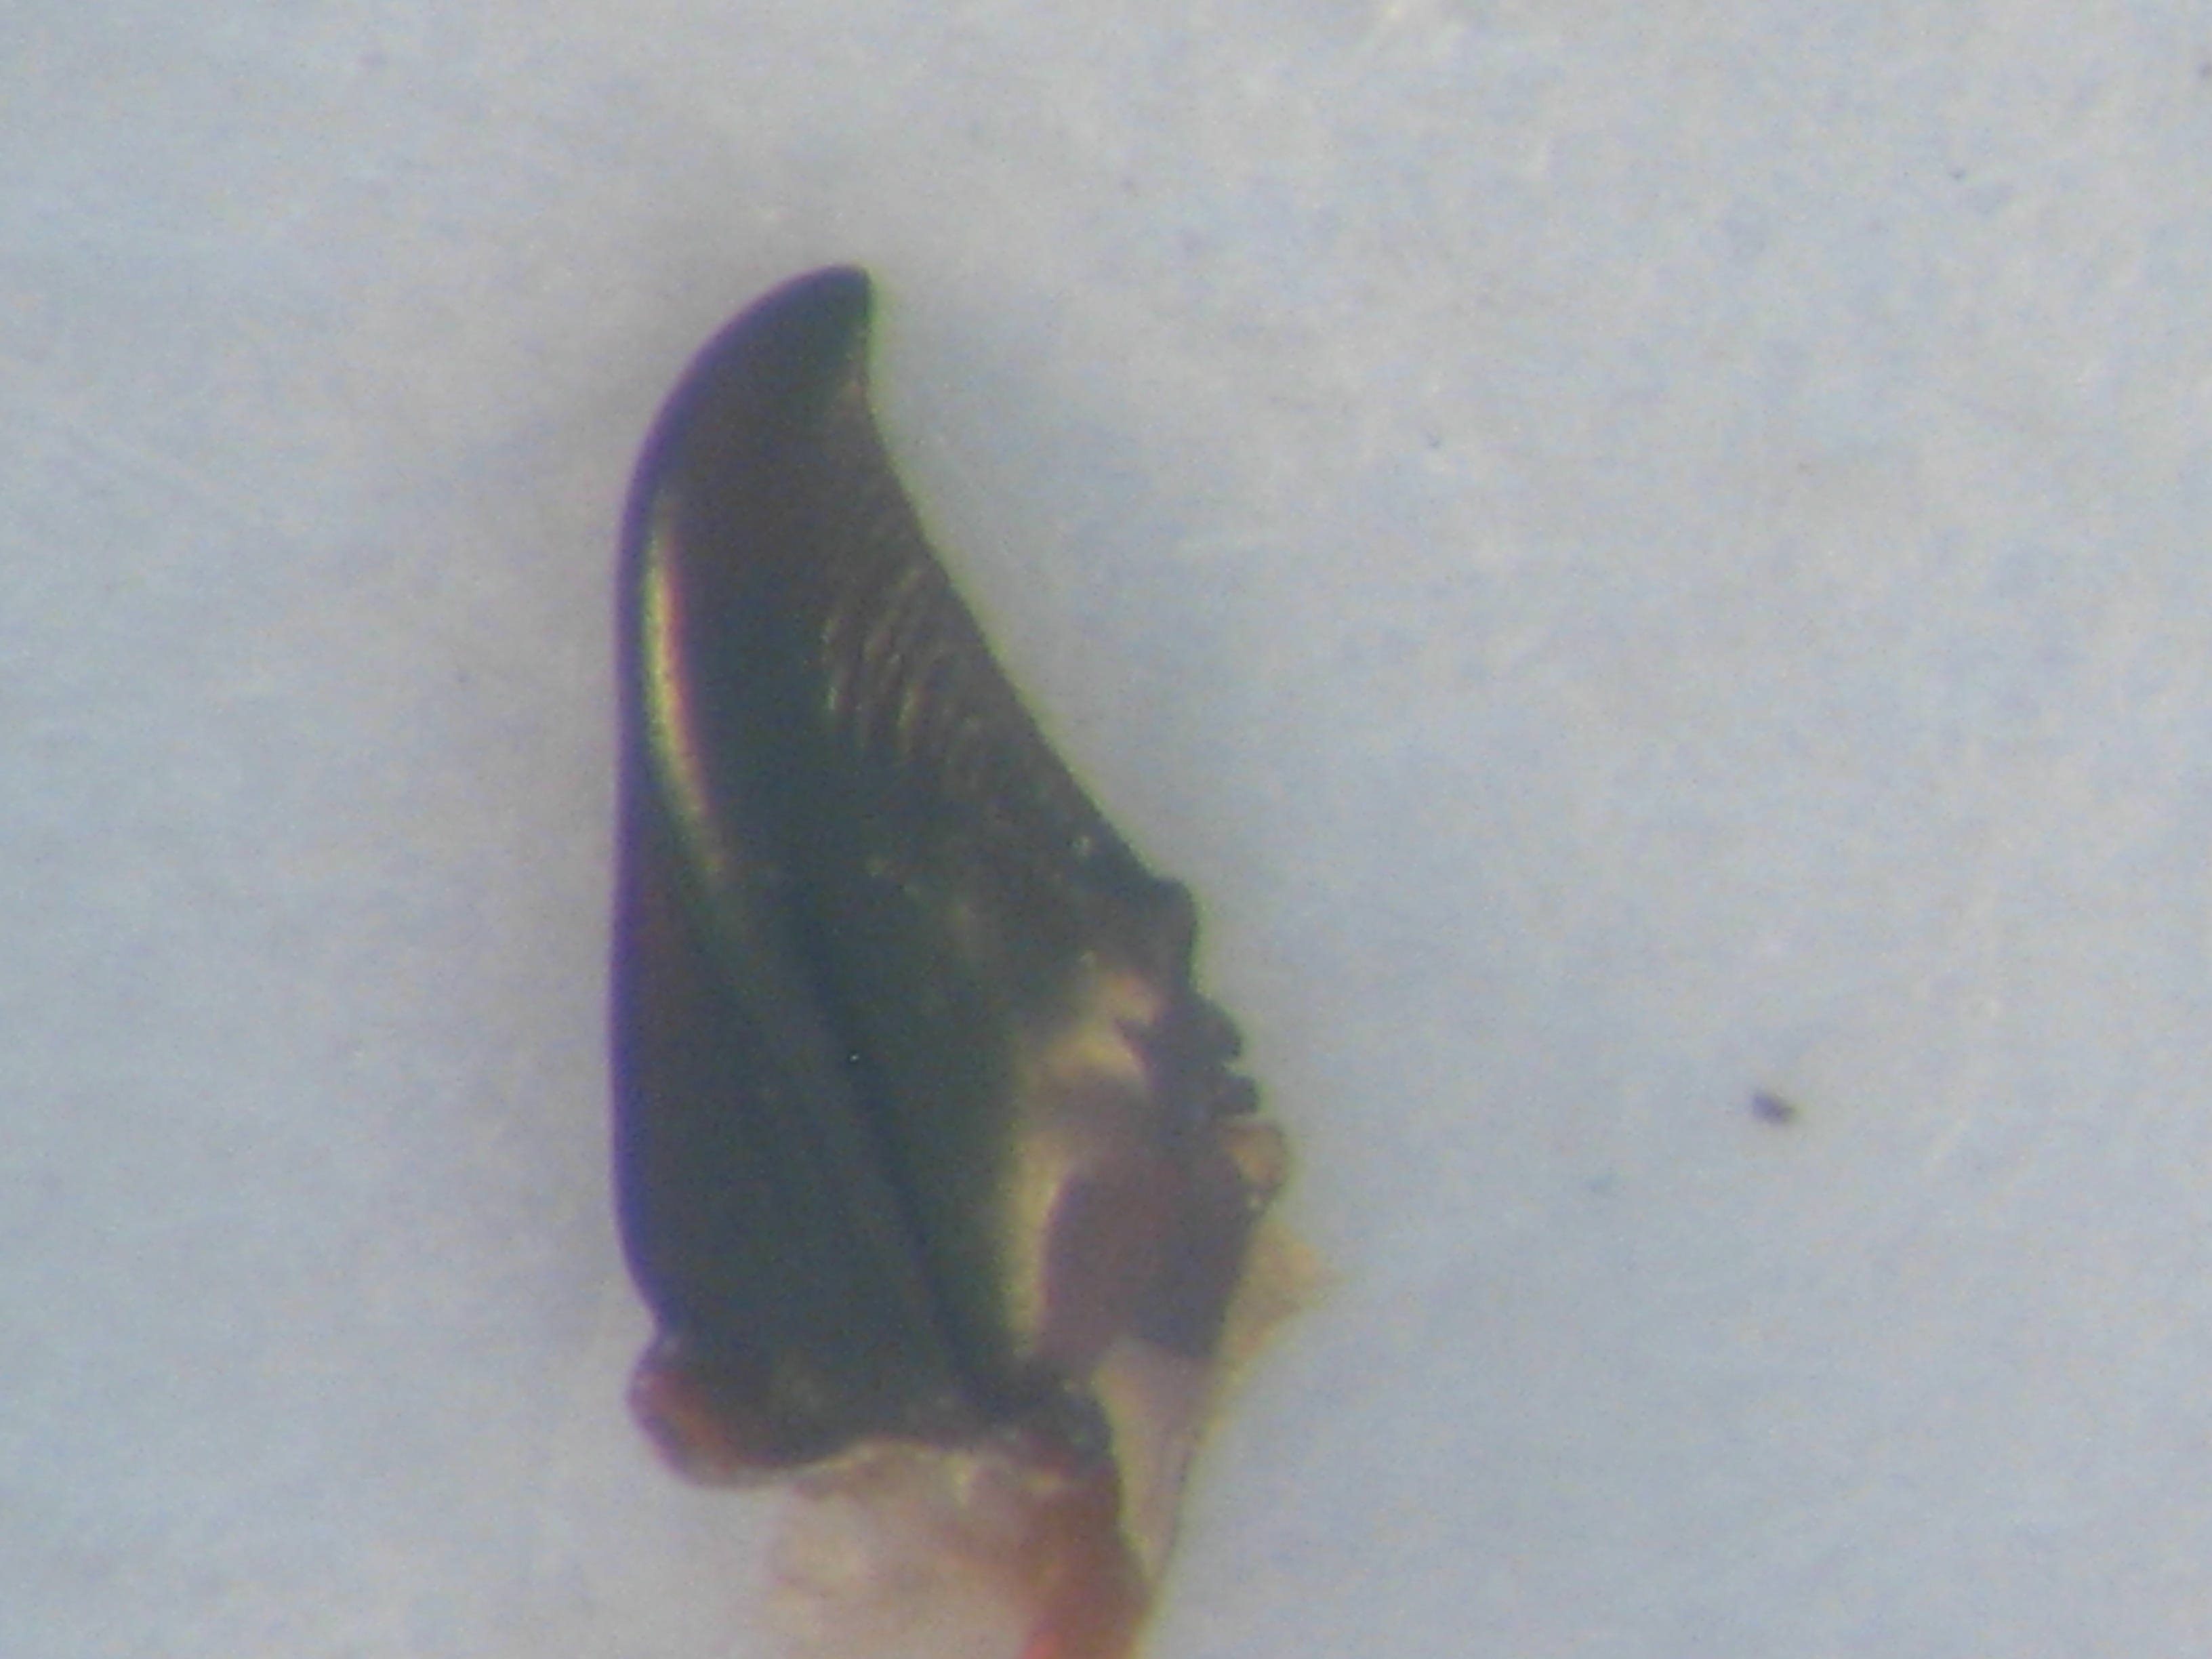
\includegraphics[width=0.22\textwidth]{./images/lm}}~~
\subfloat[Right mandible]{\label{figrbox1}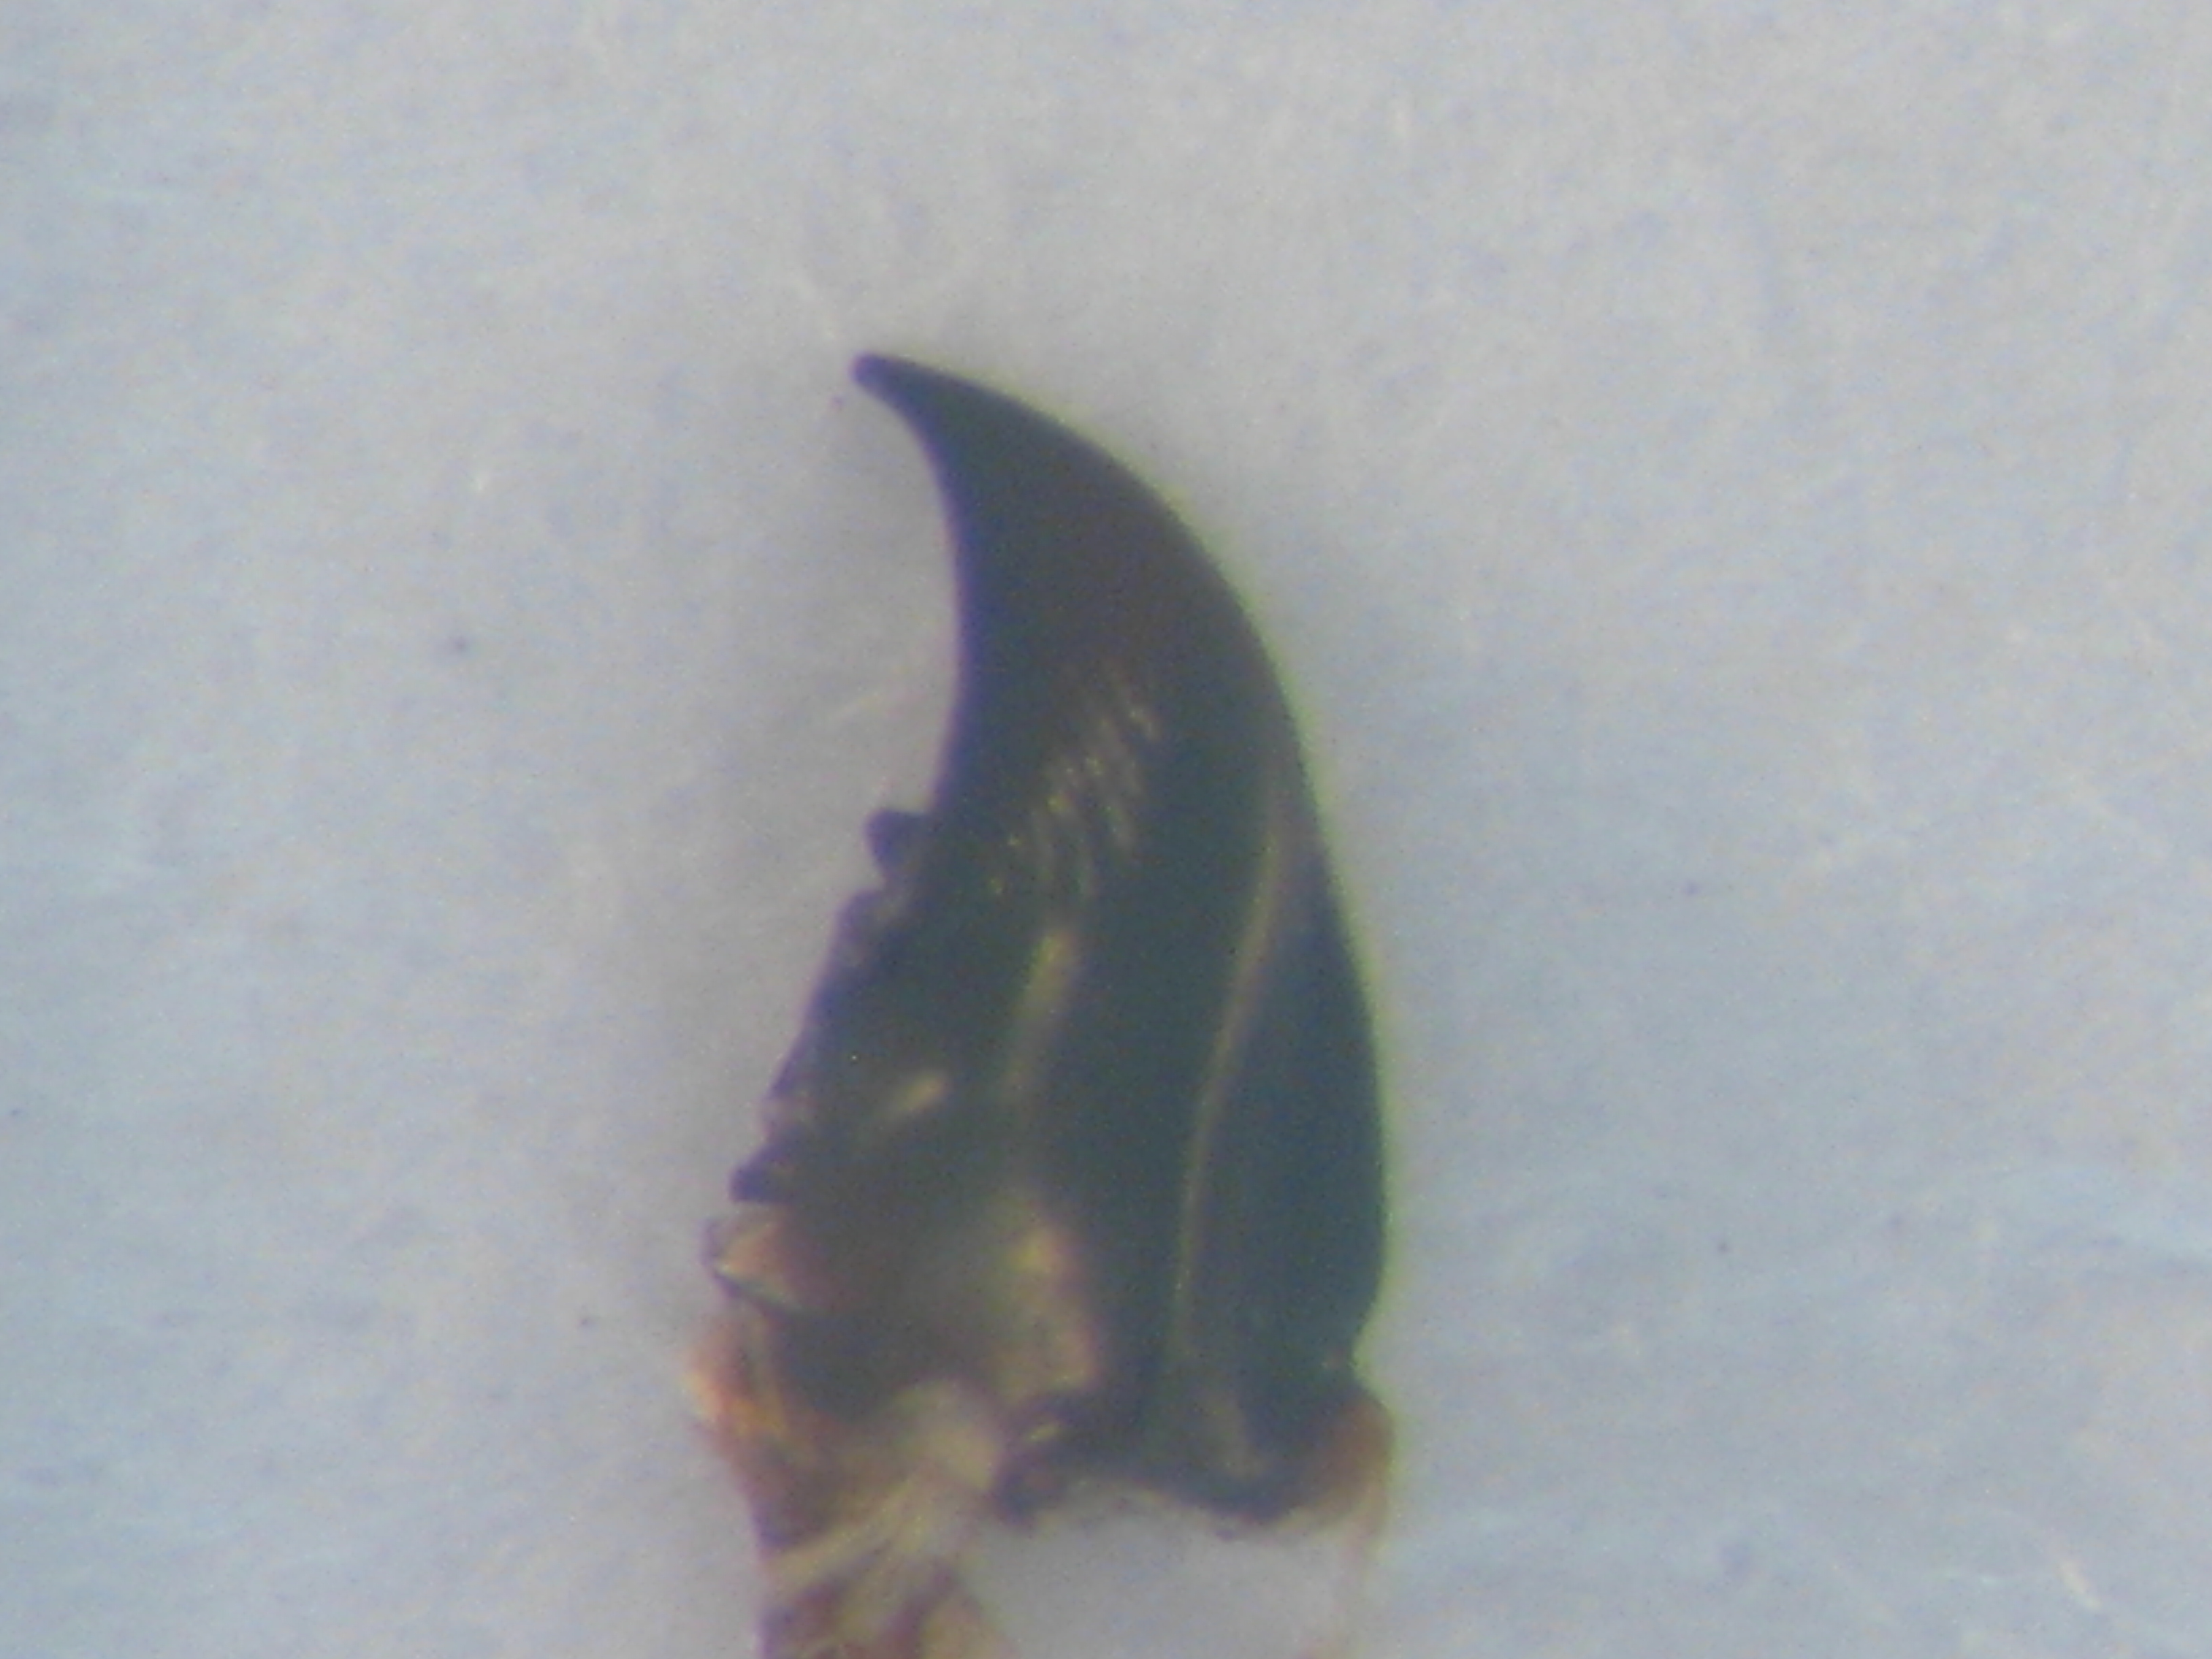
\includegraphics[width=0.22\textwidth]{./images/rm}}
\caption{Sample of pictures of beetle mandibles took by biologists.}
\label{figparts}
\end{figure}

In this paper, we focus on a chain of algorithms to automatically identify  landmarks in 2D images. The method
mainly includes three steps: firstly, a segmentation of the mandible shape,
then an iterative principal component analysis
to register a query image on a model image, and finally a
landmark estimation using the SIFT descriptor.\\

The section 2 presents the complete workflow then the section 3 details the experiments and expose the results. 


%%%%%%%%%%%%%%%%%%%%%%%%%%%%%%%%%%%%%%%%%%%%%%%%%%%%%%%%%%%%%%%%%%%%%%%%%%%%%
\section{Method}

\begin{figure}[htb]
    \centering
    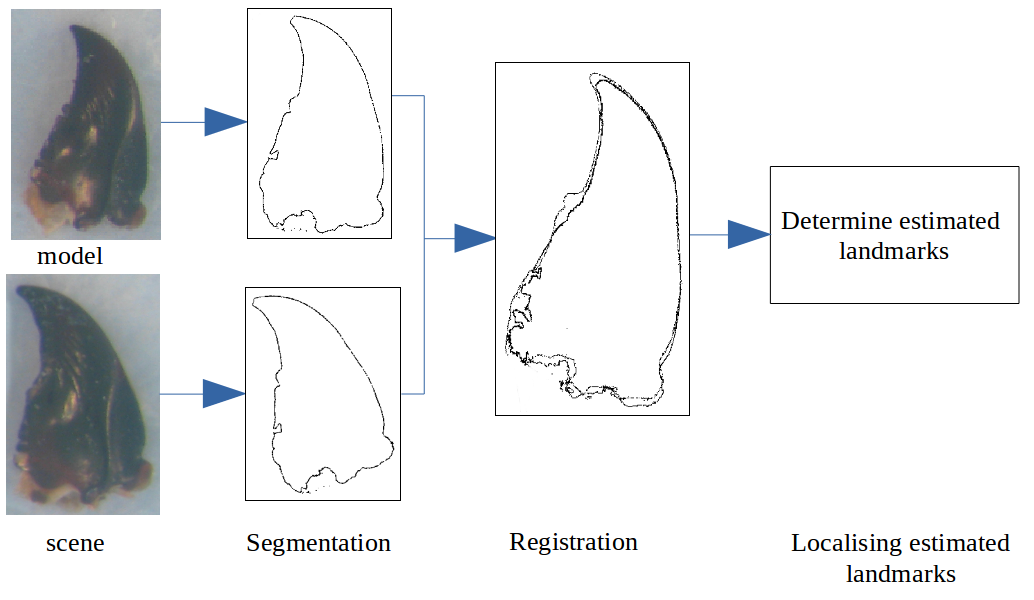
\includegraphics[width=0.5\textwidth]{./images/method}
    \caption{Overview of the proposed method}
    \label{fig:method}
\end{figure}
The addressed problem is the automatic detection of landmarks on mandible photographies to replace the manual operation by an operator.
We propose hereafter a workflow including (1) the segmentation of each image, (2) a registration step on a model image then (3) the detection of landmark positions.
The Fig. \ref{fig:method} shows the summarize the workflow.
It is worth to note that the model image is chosen randomly from the set of images without broken mandibles.
Moreover, all pictures of mandibles have been taken in the same conditions with the same camera and at the same resolution.


\subsection{Image segmentation}

The segmentation step is the first major task of a large number of image processing
chain. We have chosen a contour-based algorithm, the
Canny alogrithm \cite{canny1986computational}, allowing to determine the 
contour belonging to the shape of the mandible.
To use this method, two threshold values have to be set.
As it is mentioned in \cite{adaptiveCanny}, determine the right thresholds could be difficult.
The mandatory \textit{threshold value} used by Canny algorithm is determined by analyzing the image
histogram (see \cite{leestimating} for detail). Most often authors define these thresholds as a lower and an upper one with a usual ratio of $T_{lower} = (1/2) \times T_{upper}$.
In order to consider a larger range of values, we prefer set $T_{lower} = 1/3 \times T_{upper}$.
We can note that to optimize the computing time, the direction of the gradient of each pixel belonging to the mandible contour is computed during the Canny algorithm and will be used later.
To obtain the segmentation of the mandible, the contours obtained with Canny are discriminated to only keep the mandible contours.
As shown in Fig. \ref{canny}, the Canny algorithm generates some contours which do not belong to the mandible shape.
With a simple algorithm, the contour image is parsed to suppress the edges inside the bigger contour.
\begin{figure}[htb]
\centering
\subfloat[Contours identifying by the Canny algorithm]
  {\label{canny1}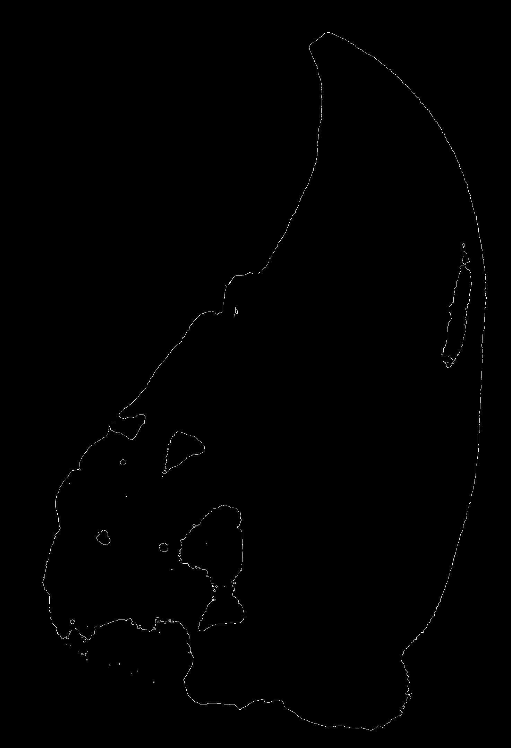
\includegraphics[width=0.2\textwidth]{./images/canny1}}~~ 
\subfloat[Contour selection by post-processing]
  {\label{canny2}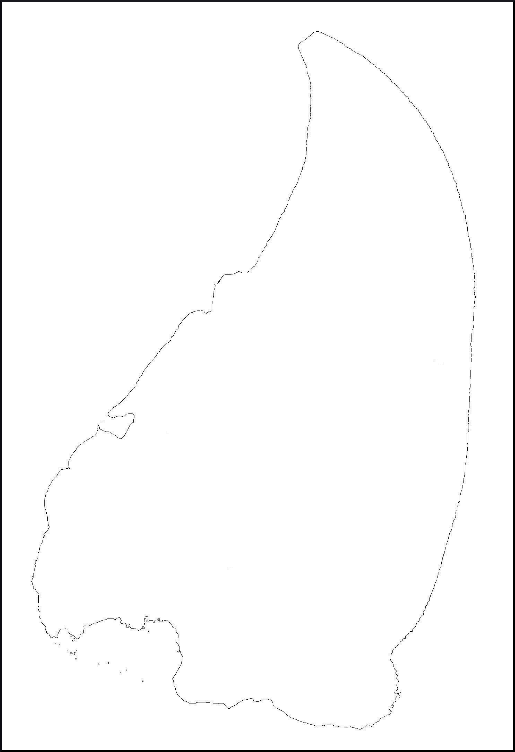
\includegraphics[width=0.2\textwidth]{./images/canny2}}
\caption{Step of the mandible contour detection.}
\label{canny}
\end{figure}


\subsection{Image registration}

As noted in introduction, all images have been captured with the same scale.
But the size of mandible can vary from a beetle to another one and/or the orientation and position can be different from a photography to another one.
The next step concerns the registration of an image on a reference image.

We have chosen to use a Principal Component Analysis (PCA) \cite{bsspca}, \cite{shlens2014tutorial} to determine the rotation and translation parameter values between the two images.
As input values, we use the lists of contour points defined at the segmentation step.
Firstly, the centroid point and principal axis of each image are defined.
The centroid point coordinates are computed like the mean coordinate of all contour points.
The principal axis is a line connecting the centroid point to a contour point, determined as detailed in algorithm \ref{alg1}.

\begin{algorithm}
	\SetKwInOut{Input}{Input}
	\SetKwInOut{Output}{Output}
	\Input{Centroid point $c$, list of contour points $l$}
	\Output{The principal axis $a$}
	\For{ all points $p_i$ in $l$ }
	{
		\For{ all points $p_j$ in $l$}
		{
			\If{$p_i \neq p_j$}
			{
				Compute the perpendicular distance $d_{ij}$ between line $(c,p_i)$ and $p_j$.
			}		
		}
		Compute the average distance ($d_{mean}$) of all distances $d_{ij}$;\\

		\If{$d_{mean}$ is minimal}
		{
			$p_{min} = p_i$;\\
		}
	}
	The principal axis is: $a = (c,p_{min})$.
	\caption{The algorithm for finding the principal axis of a list of contour points}
	\label{alg1}
\end{algorithm}

The translation is calculated like the distance between the centroid points of the scene and the model.
The rotation angle is the angle between the principal axes of these two images. Translation then rotation are applied to register the scene one the model. However, in some cases, the translation and rotation between two images are
not enough precise because the result of the segmentation could contain some noise.
To improve registration, we have enhanced the PCA by iterating until stabilization (PCAI).
We have considered some specificity of our images and observed that the tip of mandible is less noisy than its base on images.
So, we sort the contour points according to their y-value to build the subset containing the half upper part of contour points.
PCA is again completed for this subset to refine the rotation and translation values. This operation is iterated until the new computing angle is lower than 1.5 degrees (see Fig. \ref{fig:pcai}).
\begin{figure}[htb]
    \centering
    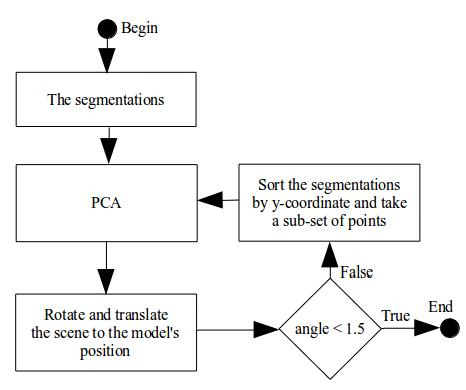
\includegraphics[width=0.45\textwidth]{./images/pcadiagram}
    \caption{The workflow of the PCAI, allowing to refine the translation and rotation values.}
    \label{fig:pcai}
\end{figure}~\\
The Fig. \ref{fig:box} shows an example of the successive results obtained with PCAI. The red contours belong to the model, the black ones are the scene contours after one iteration, and the blue ones are the resulting contours.\\

\begin{figure}[htb]
    \centering
    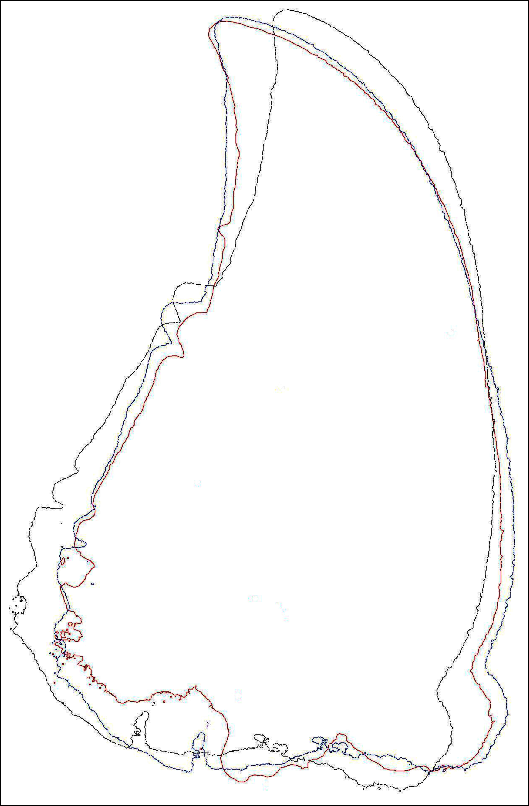
\includegraphics[width=0.3\textwidth]{./images/imreg}
    \caption{Iterations of the registration step between the model contour (in red) and the contours of the scene image.}
    \label{fig:box}
\end{figure}


\subsection{Landmark detection using SIFT}

The last task of the workflow consists in estimating the landmarks of the scene from the manual ones of the model.
We use the SIFT method \cite{lowe2004distinctive} but we do not consider all points of the image as usually, only the area around each landmark of the model.
Firstly, the region (called patch) around each landmark of the model is computed then extracted in the scene image at the same position.
Then, the SIFT descriptor is computed: the orientation and gradient magnitude are calculated for each pixel by using the gradient values computed during the Canny step by applying the following equations (\ref{eq:sift}):
%\begin{equation}
%\label{eq:sift}
%\resizebox{.5 \textwidth}{!} 
%{$
%\begin{aligned}
%	m(x,y) = \sqrt{(P(x+1,y) - P(x-1,y))^2 + (P(x,y+1) - P(x,y-1))^2} \\
%	\theta(x,y) = tan^{-1}((P(x,y+1) - P(x,y-1))/(P(x+1,y) - P(x-1,y)))
%	\end{aligned}
%$}
%\end{equation}
\begin{equation}
\label{eq:sift}
\begin{split}
	m(x,y) &= \sqrt{v_x^2 + v_y^2} \\
	\theta(x,y)& = tan^{-1}(v_y/v_x) \\
\end{split}
\end{equation}
Where:
\begin{itemize}[nosep,label=\footnotesize$\bullet$]
	\item $v_x = I(x+1,y) - I(x-1,y)$
	\item $v_y = I(x,y+1) - I(x,y-1)$
	\item $I(x,y)$ is the gray value at position $(x,y)$ in the image,
	\item $m(x,y)$ is the gradient magnitude of the pixel at position $(x,y)$,
	\item $\theta(x,y)$ is the orientation of the pixel at position $(x,y)$.
\end{itemize}
The SIFT descriptor for each patch is an histogram containing the sum of pixel gradients for each considered direction.
As usually, eight directions are taking into account ($0^o - 45^o$, $46^o - 90^o$, $91^o - 135^o$, $136^o - 180^o$, $181^o - 225^o$, $226^o - 270^o$, $271^o - 315^o$, $316^o - 360^o$). Finally, the feature vector is normalized to reduce the effects of illumination changes.

\begin{figure}[htb]
    \centering
    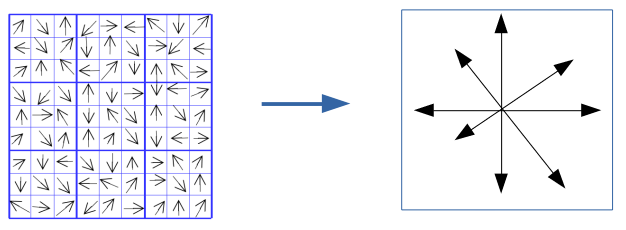
\includegraphics[width=0.4\textwidth]{./images/keypoint_descriptor}
    \caption{Calculus of the SIFT descriptor for a patch. The arrow length corresponds to the gradient value in the right figure.}
    \label{fig:kpdescriptor}
\end{figure}
The Fig. \ref{fig:kpdescriptor} shows a patch sample of 9x9 pixels centered in each landmark on the model.
The size of 9x9 has been retained after several tests.
Patch sizes 18x18, 36x36 and 54x54 have been also computed but gave unsatisfactory results.
From the patch histogram, we obtain the global gradient value for each direction.\\

The comparison between two SIFT descriptors is done by using the $L2$-distance with the following equation (\ref{eq:L2distance}):
\begin{equation}
\label{eq:L2distance}
	L(D1,D2) = \sum\limits_{i = 0}^{n}\sqrt{(D1_i-D2_i)^2}
\end{equation}
Where:
\begin{itemize}[nosep,label=\footnotesize$\bullet$]
	\item $n$ is the number of directions
	\item $D1$ and $D2$ are two descriptors of size $n$,
	\item $D1_i$ and $D2_i $ are the $i^{th}$ descriptor values.
\end{itemize}
The Fig. \ref{fig:Illustrate} illustrates how we apply SIFT into our workflow.
To detect the scene landmarks, the patches \textit{$P_m$} of the model and \textit{$P_s$} of the scene are created with the size of $P_m$ smaller than the size of $P_s$.
After experiments, we have kept 36 pixels as the size of \textit{$P_s$}.
For each pixel in the patch \textit{$P_s$}, a sub-patch \textit{$P'_s$} is extracted with the same size than \textit{$P_m$}.
When the \textit{$P'_s$} have a part outside \textit{$P_s$}, the outside pixels are also considered.
Then, the distance \textit{$L(P_m,P'_s)$} is computed using equation (\ref{eq:L2distance}).
The position of the estimated landmark corresponds to the position of the sub-patch \textit{$P'_s$} with the smallest distance $L$ to \textit{$P_m$}.
Finally, the position of the estimated landmarks are set in the original location of the original scene image by applying the reverse operation of rotation and translation.
\begin{figure}[htb]
    \centering
    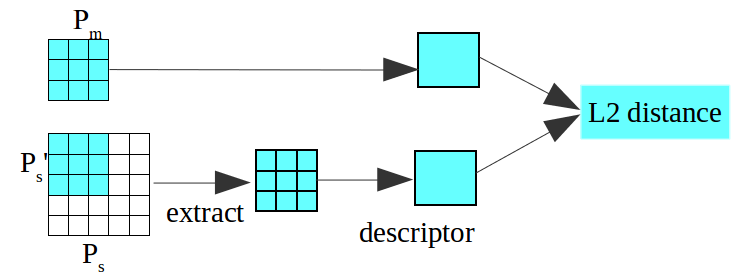
\includegraphics[width=0.48\textwidth]{./images/illustration_SIFT}
    \caption{Steps of descriptors comparisons between the patch $P_m$ of the model image and the patches $P'_s$ of the scene image.}
    \label{fig:Illustrate}
\end{figure}


\section{Experiments and result}

The complete method is implemented in MAELab\footnote{MAELab
  is a free software written in C++. It can be directly and freely obtained by request
  at the authors.}.
The beetles has been analyzed after a split in right and left mandible sets.
After verifying the quality of the image, it remains 290 usable images of right mandibles and 286 images of left mandibles.
The removed images include the images without mandible or with broken mandibles.
In all valid images, a set of manual landmarks is indicated by biologists: 18 for right mandibles, 16 for left mandibles.

We have run the full workflow on all the usable images.
The results have shown differences in algorithm accuracy: estimated landmarks are well positioned on some scene images but not satisfying on others.
As we mentioned before, mandibles images can exhibit different sizes because beetles have also different sizes of mandible.
We detected that our method is sensible to this parameter.
To improve the results, we have inserted a pre-processing step before the computing of the SIFT descriptors to estimate the scale between a scene image and the model.
The bounding boxes of the mandible of the model image and the scene image are computed and the scales in the x- and y-directions are determined by the ratio between the corresponding sides of the bounding boxes.
Then, the scene contours are rescaled to fit the model contours. \\
\begin{figure}[h]
\centering
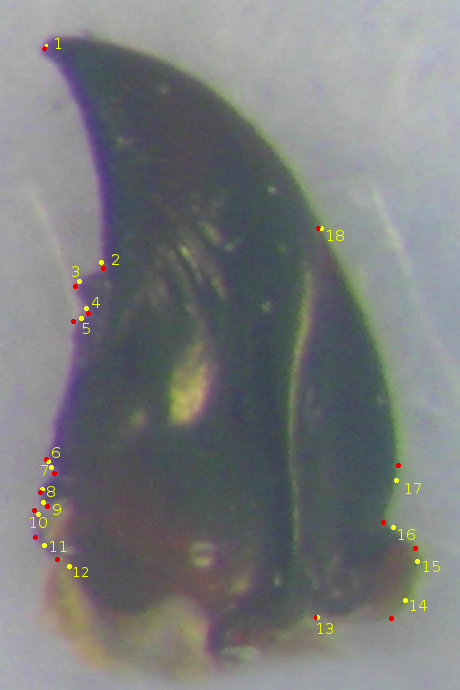
\includegraphics[width=0.35\textwidth]{./images/md_rs}
\caption{The manual (in red) and estimated (in yellow) landmarks on a right mandible.}
\label{figresult}
\end{figure}~\\
\begin{figure}[h]
\centering
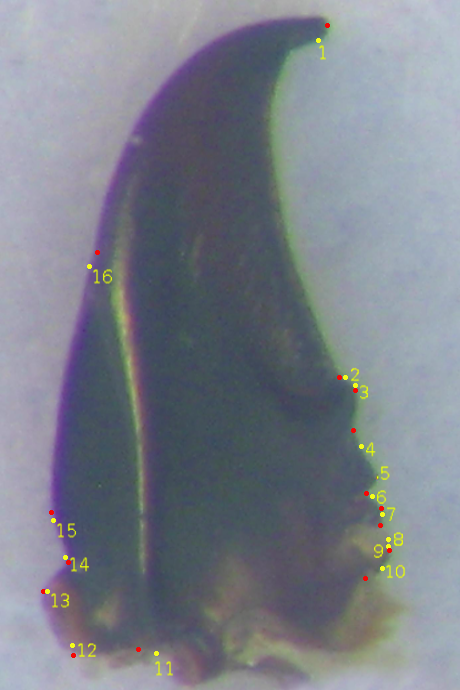
\includegraphics[width=0.35\textwidth]{./images/mg_rs}
\caption{The manual (in red) and estimated (in yellow) landmarks of a left mandible.}
\label{figresult2}
\end{figure}

The Figs. \ref{figresult} and \ref{figresult2} show the final results for a right and a left mandible with the manual and estimated landmarks.
The estimated landmarks are quite near with the manual landmarks, as you can see with the following statistical evaluation.

The statistic are obtained for all landmarks of the scene images.
We have compared the positions between the manual and estimated landmarks by accepting an error from 1\% to 2\% of the bounding box's size.
According to this way, a global statistic compares all pairs of corresponding landmarks on all images as presented in Fig. \ref{figctresult}.
It shows the global results with a score of well positioned landmarks equal to \textbf{87.03}\% for right mandibles and \textbf{78.82}\% for left mandibles.
\begin{figure}[h]
\centering
\subfloat[Set of right mandibles.]{\label{figmdresult}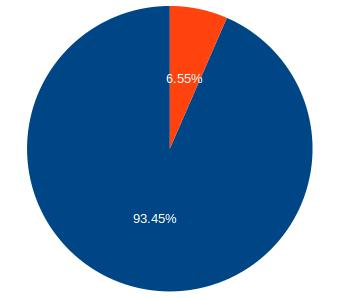
\includegraphics[width=0.22\textwidth]{./images/mdresult}}~~
\subfloat[Set of left mandibles.]{\label{figmgresult}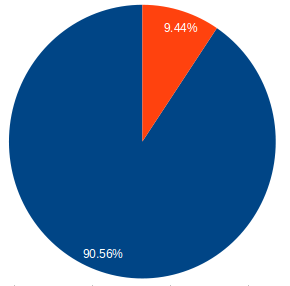
\includegraphics[width=0.22\textwidth]{./images/mgresult}}
\caption{The mean proportion of well and bad landmark locations of the two sets of left and right mandibles.}
\label{figctresult}
\end{figure}

Besides the global results, we are also interested by the accuracy of the individual positions of the estimated landmarks.
We have computed the distance between the manual landmarks and their corresponding estimated landmarks in order to examine the proportion of well positioned landmarks.
The Fig. \ref{figmdresultlm} and \ref{figmgresultlm} show the proportion of well estimated landmarks for each landmark of the model.
With 18 landmarks of right mandible, the position of the $1^{st}$ estimated landmarks is very accurate with \textbf{98.62}\%.
The lowest proportion is \textbf{74,48}\% for the $14^{th}$ landmark.
The remaining landmarks are also estimated with a accuracy greater than 75\%.
For left mandibles, the highest and lowest success rates are \textbf{93,01}\% for the $1^{st}$ landmark and \textbf{60,14}\% for the $16^{th}$ landmark.
The statistic is done on each estimated landmark of all the images with a standard deviation error \cite{bland1996statistics}.
As we can see in Fig. \ref{canny}, the noise of the contour part located at the base of a mandible is higher than the noise located at the tip of the mandible.
This explains why the correct proportion on $11^{th}$ and $12^{th}$ landmark of the left mandible and $13^{th}$ and $14^{th}$ landmark of the right mandible are less accurate than other landmarks.
Moreover, when we reconsider the datasets, the left mandible images have bigger scale values than the right mandible images.
This explains than the success rate on the right mandibles is always greater than on the left mandibles in all experiments.
\begin{figure}[htb]
    \centering
    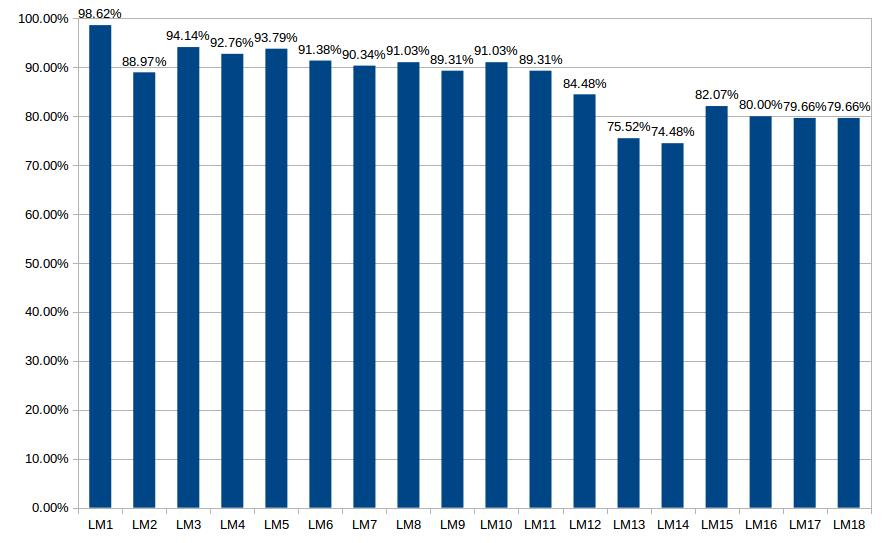
\includegraphics[width=0.5\textwidth]{./images/md_chartlms}
    \caption{The proportions of well estimated landmark for each model landmark of right mandibles.}
    \label{figmdresultlm}
\end{figure}
\begin{figure}[htb]
    \centering
    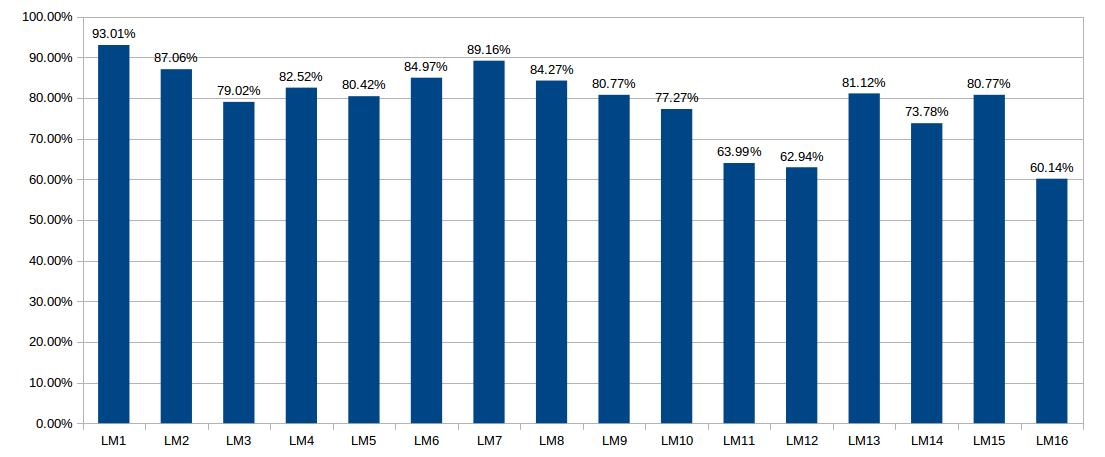
\includegraphics[width=0.5\textwidth]{./images/mg_chartlms}
    \caption{The proportions of well estimated landmark for each model landmark of left mandibles.}
    \label{figmgresultlm}
\end{figure}

\section{Conclusion}

The morphometric analysis is a powerful tool in biology for the beetle species classification.
In this paper, we have design a method to segment their mandibles and automatically locate landmarks which have been determined on a model by biologists.
Each mandible has been segmented by using the Canny algorithm before to be registered using PCAI to align the images.
The estimation step of the landmark position use the SIFT descriptor to find the best matching position.
The results show that the method succeed in locating the landmarks for all images.
The accuracy of the method is sufficient to be proposed to biologists as a replacement of the manual measures, but with a manual check for the bottom landmark.
Moreover, considering the previous work in \cite{leestimating}, this method reduces the drastically the number of outlier landmarks and the MAELab implementation also reduce the global computing times and memory cost.
From now, the next stage consists in improving the registration step in order to increase the matching step accuracy and completely remove manual interventions.
By example, we could investigate the isomorphic registration methods to be more robust to the inter-species variations of mandible shapes.




\bibliographystyle{plain}
\bibliography{references}

\end{document}

%-------------------------------------------------------------------------
% example of algorithm typesetting
% to allow this, uncomment line 
% \RequirePackage[noend]{myalgorithm}
% in the wscg.sty file
% and download that package from Gabriel Zachmann's page http://zach.in.tu-clausthal.de/latex/
%
%
%\begin{algorithm}
%\hrule
%  \centering
%\begin{algorithmic}
%    \STMT $d_{l,r} = f_B(P_1), f_B(P_n)$
%    \WHILE{ $|d_l| > \epsilon $ and $|d_r| > \epsilon $ and $l<r$}
%        \STMT $d_x = f_B(P_x)$
%        \IF{ $d_x < 0$ }
%            \STMT $l, r = x, r$
%        \ELSE
%            \STMT $l, r = l, x$
%        \ENDIF
%    \ENDWHILE
%\end{algorithmic}
%\hrule
%\caption{Example of some pseudo-code}
%\label{fg:code}
%\end{algorithm}

%-------------------------------------------------------------------------

\begin{thebibliography}{99}
\label{references}
\bibitem[1]{canny} Canny, John. "A computational approach to edge detection." IEEE Transactions on pattern analysis and machine intelligence 6 (1986): 679-698.
\bibitem[2]{Ballard} Ballard, Dana H. "Generalizing the Hough transform to detect arbitrary shapes." Pattern recognition 13.2 (1981): 111-122.
\bibitem[3]{Webster} Webster, M. A. R. K., and H. DAVID Sheets. "A practical introduction to landmark-based geometric morphometrics." Quantitative Methods in Paleobiology 16 (2010): 168-188.
\bibitem[4]{est} Le Van, L., et al. "Estimating landmarks on 2D images of beetle mandibles."
\bibitem[5]{pca} Shlens, Jonathon. "A tutorial on principal component analysis." arXiv preprint arXiv:1404.1100 (2014).
\bibitem[6]{sift} Lowe, David G. "Distinctive image features from scale-invariant keypoints." International journal of computer vision 60.2 (2004): 91-110.
\bibitem[7]{palaniswamy} Palaniswamy, Sasirekha, Neil A. Thacker, and Christian Peter Klingenberg. "Automatic identification of landmarks in digital images." IET Computer Vision 4.4 (2010): 247-260.
\end{thebibliography}

%{\bfseries
%Last page should be fully used by text, figures etc. Do not leave empty space, please. 

%Do not lock the PDF -- additional text and info will be inserted, i.e. ISSN/ISBN etc. 
%}

